\begin{appendices}
    \section{Implementation} \label{sec:Implementation}
    The code can be found here[]. \\
    Both the Identification and the Pricing Problem were programmed in Python 2.7 using NumPy 1.12.1, SciPy 0.19.1 and PyTorch 0.1.12 modules [web cites] \cite{SCPOptimizeDocs}\cite{NPDocs}. [Results from Python plotted in Matplotlib 2.0.2] With some code optimizations, the input dataset $\matr{F}$ was built using NumPy's \texttt{ndarray} and PyTorch's \texttt{tensor} functions. Since PyTorch offers NumPy-like code base but with dedicated neural network functions and submodules, PyTorch's \texttt{relu} and \texttt{softmax} functions were used along with other matrix operations.\\
    
    \subsection{Specific Implementation Details for the Pricing Problem}
    Among all the code optimizations in both models, some in that for the Pricing Problem are worth discussing, as they drastically differ from Algorithm \ref{alg:Solving the Pricing Problem} or are intricate. Most optimizations relevant to the Identification Problem are trivial and relate directly to those for the Pricing Problem. Therefore, only those in the Pricing Problem model are discussed.
    
    \subsubsection{Building the Dataset $\matr{F}$}
    Notice that we build the dataset $\matr{F}$ and batch-multiply it with $\matr{w_1}$ on each iteration/epoch (lines 2-3 of Algorithm \ref{alg:Solving the Pricing Problem}). Doing these steps are repetitive as most elements of $\matr{F}$, distances $\matr{D}$ and environmental feature vector $\vect{f}$, do not change unlike rewards $\vect{r}$. Moreover since $\matr{w_1}$ is fixed, Algorithm \ref{alg:Solving the Pricing Problem} would repetitively multiply the $\vect{f}$ and $\matr{D}$ components of $\matr{F}$ with $\matr{w_1}$. To avoid these unnecessary computations, we preprocessed most of $\matr{F}$ by batch-multiplying with $\matr{w_1}$ and only multiplied $\vect{r}$ with the corresponding elements of $\matr{w_1}$. Figure \ref{fig:Splitting and Batch Multiplying F and w1} describes the process graphically.\\
    \begin{figure}[!htbp]
        \centering
        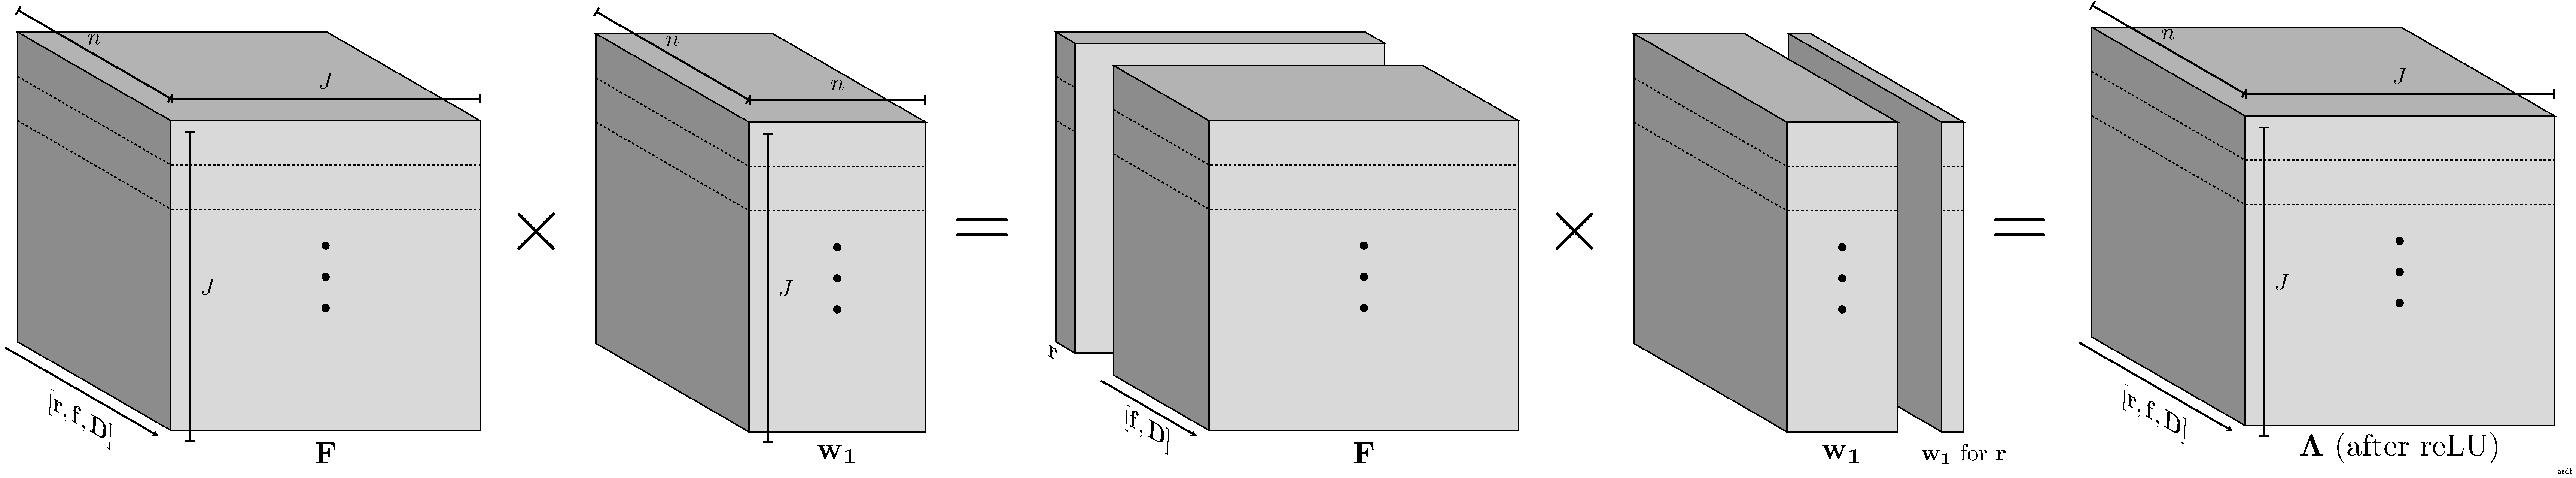
\includegraphics[width=\linewidth]{split_and_batch_multiply}
        \caption{Splitting and Batch Multiplying $\matr{F}$ \& $\matr{w_1}$}
        \label{fig:Splitting and Batch Multiplying F and w1}
    \end{figure}    
    Although this preprocessing might seem applicable for the model in Identification Problem too, it does not apply fully. Since the weights $\matr{w_1}$ are updated on each iteration/epoch, we cannot multiply them with parts of $\matr{F}$ beforehand (Algorithm \ref{alg:Algorithm for the Identification Problem}). However, we can combine $\matr{D}$ and $\vect{f}$ in the preprocessing stage and simply append $\vect{r}[t]$ on each iteration, saving computation time.
    
    \subsubsection{Modeling the Linear Programming Problem in the Standard Format}
    The \texttt{scipy.optimize} module's \texttt{linprog} function requires that the arguments are in standard LP format. As discussed in \cref{sec:Calculating Rewards}, Equation \ref{eq:lp_code_constrain_rewards} resembles the standard format more closely than \ref{eq:lp_math_constrain_rewards}, but it may not be clear how so.\\
    
    Considering $\vect{u}$ and $\vect{r'}$ as variables $\vect{x}$, Equation \ref{eq:lp_code_constrain_rewards} translates into Equation \ref{eq:lp_matrix_rewards} ($J$ is the number of locations).
    \begin{equation} \label{eq:lp_matrix_rewards}
    \begin{aligned}
    & \text{minimize}
    & & \begin{bmatrix}
    \vect{0_J}\\
    \vect{1_J}\\
    \end{bmatrix}^T
    \begin{bmatrix}
    \vect{r'}\\
    \vect{u}
    \end{bmatrix}\\ \\
    & \text{subject to}
    & & \begin{bmatrix}
    I_J & -I_J\\
    -I_J & -I_J\\
    \vect{1}^T_J & \vect{0}^T_J\\
    \end{bmatrix}
    \begin{bmatrix}
    \vect{r'}\\
    \vect{u}\\
    \end{bmatrix} \leq
    \begin{bmatrix}
    \vect{r}\\
    -\vect{r}\\
    \mathcal{R}\\
    \end{bmatrix}\\
    &&& r'_i, u_i \geq 0
    \end{aligned}
    \end{equation}
    
    \section{Strange GPU Speedup in LP Computation} \label{sec:Strange GPU Speedup in LP Computation}
    Furthermore, although we expected SciPy's Optimize Module \cite{SCPOptimizeDocs} to run on the CPU (see \cref{sec:Pricing Problem-Testing GPU Speedup on the Random Dataset}), the LP problem ran faster when the GPU was ``set''. We did not anticipate this behavior, and we couldn't pick out a reason for the Optimize Module supposedly doing operations differently. Since our GPU ``set'' and CPU ``set'' configurations were only enforceable on user-created functions and datasets, we do not know why the LP solver delivered different speeds while solving the same problem. If it used the CPU or the GPU, it should have done so in both cases and the runtime would have been equal. While there could be differences in implementation, we cannot affirm or deny any reason behind this quirky behavior. Figure \ref{fig:Finding Rewards - Time taken by the LP} shows the unexpected speedup of $\frac{2.35}{1.41} \approx 1.66$x delivered by SciPy Optimize Module's LP solver.
    
    There could have been many reasons for this bizarre behavior, including but not limited to:
    \begin{itemize}
        \item SciPy's Optimize Module differentiating between configurations. This can be ruled out because the module could not have known the configuration during which it was called. That is just supernatural.
        \item 
    \end{itemize}
\end{appendices}